\documentclass[conference]{IEEEtran}
% Add the compsoc option for Computer Society conferences.
%
% If IEEEtran.cls has not been installed into the LaTeX system files,
% manually specify the path to it like:
% \documentclass[conference]{../sty/IEEEtran}

% TODO: ok?

\usepackage{tabularx}
\usepackage{tabulary}

% Some very useful LaTeX packages include:
% (uncomment the ones you want to load)


% *** MISC UTILITY PACKAGES ***
%
%\usepackage{ifpdf}
% Heiko Oberdiek's ifpdf.sty is very useful if you need conditional
% compilation based on whether the output is pdf or dvi.
% usage:
% \ifpdf
%   % pdf code
% \else
%   % dvi code
% \fi
% The latest version of ifpdf.sty can be obtained from:
% http://www.ctan.org/tex-archive/macros/latex/contrib/oberdiek/
% Also, note that IEEEtran.cls V1.7 and later provides a builtin
% \ifCLASSINFOpdf conditional that works the same way.
% When switching from latex to pdflatex and vice-versa, the compiler may
% have to be run twice to clear warning/error messages.






% *** CITATION PACKAGES ***
%
%\usepackage{cite}
% cite.sty was written by Donald Arseneau
% V1.6 and later of IEEEtran pre-defines the format of the cite.sty package
% \cite{} output to follow that of IEEE. Loading the cite package will
% result in citation numbers being automatically sorted and properly
% "compressed/ranged". e.g., [1], [9], [2], [7], [5], [6] without using
% cite.sty will become [1], [2], [5]--[7], [9] using cite.sty. cite.sty's
% \cite will automatically add leading space, if needed. Use cite.sty's
% noadjust option (cite.sty V3.8 and later) if you want to turn this off.
% cite.sty is already installed on most LaTeX systems. Be sure and use
% version 4.0 (2003-05-27) and later if using hyperref.sty. cite.sty does
% not currently provide for hyperlinked citations.
% The latest version can be obtained at:
% http://www.ctan.org/tex-archive/macros/latex/contrib/cite/
% The documentation is contained in the cite.sty file itself.






% *** GRAPHICS RELATED PACKAGES ***
%
\ifCLASSINFOpdf
  \usepackage[pdftex]{graphicx}
  % declare the path(s) where your graphic files are
  % \graphicspath{{../pdf/}{../jpeg/}}
  % and their extensions so you won't have to specify these with
  % every instance of \includegraphics
  % \DeclareGraphicsExtensions{.pdf,.jpeg,.png}
\else
  % or other class option (dvipsone, dvipdf, if not using dvips). graphicx
  % will default to the driver specified in the system graphics.cfg if no
  % driver is specified.
  % \usepackage[dvips]{graphicx}
  % declare the path(s) where your graphic files are
  % \graphicspath{{../eps/}}
  % and their extensions so you won't have to specify these with
  % every instance of \includegraphics
  % \DeclareGraphicsExtensions{.eps}
\fi
% graphicx was written by David Carlisle and Sebastian Rahtz. It is
% required if you want graphics, photos, etc. graphicx.sty is already
% installed on most LaTeX systems. The latest version and documentation can
% be obtained at: 
% http://www.ctan.org/tex-archive/macros/latex/required/graphics/
% Another good source of documentation is "Using Imported Graphics in
% LaTeX2e" by Keith Reckdahl which can be found as epslatex.ps or
% epslatex.pdf at: http://www.ctan.org/tex-archive/info/
%
% latex, and pdflatex in dvi mode, support graphics in encapsulated
% postscript (.eps) format. pdflatex in pdf mode supports graphics
% in .pdf, .jpeg, .png and .mps (metapost) formats. Users should ensure
% that all non-photo figures use a vector format (.eps, .pdf, .mps) and
% not a bitmapped formats (.jpeg, .png). IEEE frowns on bitmapped formats
% which can result in "jaggedy"/blurry rendering of lines and letters as
% well as large increases in file sizes.
%
% You can find documentation about the pdfTeX application at:
% http://www.tug.org/applications/pdftex





% *** MATH PACKAGES ***
%
\usepackage[cmex10]{amsmath}
% A popular package from the American Mathematical Society that provides
% many useful and powerful commands for dealing with mathematics. If using
% it, be sure to load this package with the cmex10 option to ensure that
% only type 1 fonts will utilized at all point sizes. Without this option,
% it is possible that some math symbols, particularly those within
% footnotes, will be rendered in bitmap form which will result in a
% document that can not be IEEE Xplore compliant!
%
% Also, note that the amsmath package sets \interdisplaylinepenalty to 10000
% thus preventing page breaks from occurring within multiline equations. Use:
%\interdisplaylinepenalty=2500
% after loading amsmath to restore such page breaks as IEEEtran.cls normally
% does. amsmath.sty is already installed on most LaTeX systems. The latest
% version and documentation can be obtained at:
% http://www.ctan.org/tex-archive/macros/latex/required/amslatex/math/





% *** SPECIALIZED LIST PACKAGES ***
%
\usepackage[longend,linesnumbered,figure]{algorithm2e}
\usepackage{algorithmic}


\newcommand{\code}[1]{\lstset{basicstyle=\small\tt}\lstinline£#1£\lstset
{basicstyle=\footnotesize\tt}}

% algorithmic.sty was written by Peter Williams and Rogerio Brito.
% This package provides an algorithmic environment fo describing algorithms.
% You can use the algorithmic environment in-text or within a figure
% environment to provide for a floating algorithm. Do NOT use the algorithm
% floating environment provided by algorithm.sty (by the same authors) or
% algorithm2e.sty (by Christophe Fiorio) as IEEE does not use dedicated
% algorithm float types and packages that provide these will not provide
% correct IEEE style captions. The latest version and documentation of
% algorithmic.sty can be obtained at:
% http://www.ctan.org/tex-archive/macros/latex/contrib/algorithms/
% There is also a support site at:
% http://algorithms.berlios.de/index.html
% Also of interest may be the (relatively newer and more customizable)
% algorithmicx.sty package by Szasz Janos:
% http://www.ctan.org/tex-archive/macros/latex/contrib/algorithmicx/




% *** ALIGNMENT PACKAGES ***
%
%\usepackage{array}
% Frank Mittelbach's and David Carlisle's array.sty patches and improves
% the standard LaTeX2e array and tabular environments to provide better
% appearance and additional user controls. As the default LaTeX2e table
% generation code is lacking to the point of almost being broken with
% respect to the quality of the end results, all users are strongly
% advised to use an enhanced (at the very least that provided by array.sty)
% set of table tools. array.sty is already installed on most systems. The
% latest version and documentation can be obtained at:
% http://www.ctan.org/tex-archive/macros/latex/required/tools/


%\usepackage{mdwmath}
%\usepackage{mdwtab}
% Also highly recommended is Mark Wooding's extremely powerful MDW tools,
% especially mdwmath.sty and mdwtab.sty which are used to format equations
% and tables, respectively. The MDWtools set is already installed on most
% LaTeX systems. The lastest version and documentation is available at:
% http://www.ctan.org/tex-archive/macros/latex/contrib/mdwtools/


% IEEEtran contains the IEEEeqnarray family of commands that can be used to
% generate multiline equations as well as matrices, tables, etc., of high
% quality.


%\usepackage{eqparbox}
% Also of notable interest is Scott Pakin's eqparbox package for creating
% (automatically sized) equal width boxes - aka "natural width parboxes".
% Available at:
% http://www.ctan.org/tex-archive/macros/latex/contrib/eqparbox/





% *** SUBFIGURE PACKAGES ***
%\usepackage[tight,footnotesize]{subfigure}
% subfigure.sty was written by Steven Douglas Cochran. This package makes it
% easy to put subfigures in your figures. e.g., "Figure 1a and 1b". For IEEE
% work, it is a good idea to load it with the tight package option to reduce
% the amount of white space around the subfigures. subfigure.sty is already
% installed on most LaTeX systems. The latest version and documentation can
% be obtained at:
% http://www.ctan.org/tex-archive/obsolete/macros/latex/contrib/subfigure/
% subfigure.sty has been superceeded by subfig.sty.



%\usepackage[caption=false]{caption}
%\usepackage[font=footnotesize]{subfig}
% subfig.sty, also written by Steven Douglas Cochran, is the modern
% replacement for subfigure.sty. However, subfig.sty requires and
% automatically loads Axel Sommerfeldt's caption.sty which will override
% IEEEtran.cls handling of captions and this will result in nonIEEE style
% figure/table captions. To prevent this problem, be sure and preload
% caption.sty with its "caption=false" package option. This is will preserve
% IEEEtran.cls handing of captions. Version 1.3 (2005/06/28) and later 
% (recommended due to many improvements over 1.2) of subfig.sty supports
% the caption=false option directly:
%\usepackage[caption=false,font=footnotesize]{subfig}
%
% The latest version and documentation can be obtained at:
% http://www.ctan.org/tex-archive/macros/latex/contrib/subfig/
% The latest version and documentation of caption.sty can be obtained at:
% http://www.ctan.org/tex-archive/macros/latex/contrib/caption/




% *** FLOAT PACKAGES ***
%
%\usepackage{fixltx2e}
% fixltx2e, the successor to the earlier fix2col.sty, was written by
% Frank Mittelbach and David Carlisle. This package corrects a few problems
% in the LaTeX2e kernel, the most notable of which is that in current
% LaTeX2e releases, the ordering of single and double column floats is not
% guaranteed to be preserved. Thus, an unpatched LaTeX2e can allow a
% single column figure to be placed prior to an earlier double column
% figure. The latest version and documentation can be found at:
% http://www.ctan.org/tex-archive/macros/latex/base/



%\usepackage{stfloats}
% stfloats.sty was written by Sigitas Tolusis. This package gives LaTeX2e
% the ability to do double column floats at the bottom of the page as well
% as the top. (e.g., "\begin{figure*}[!b]" is not normally possible in
% LaTeX2e). It also provides a command:
%\fnbelowfloat
% to enable the placement of footnotes below bottom floats (the standard
% LaTeX2e kernel puts them above bottom floats). This is an invasive package
% which rewrites many portions of the LaTeX2e float routines. It may not work
% with other packages that modify the LaTeX2e float routines. The latest
% version and documentation can be obtained at:
% http://www.ctan.org/tex-archive/macros/latex/contrib/sttools/
% Documentation is contained in the stfloats.sty comments as well as in the
% presfull.pdf file. Do not use the stfloats baselinefloat ability as IEEE
% does not allow \baselineskip to stretch. Authors submitting work to the
% IEEE should note that IEEE rarely uses double column equations and
% that authors should try to avoid such use. Do not be tempted to use the
% cuted.sty or midfloat.sty packages (also by Sigitas Tolusis) as IEEE does
% not format its papers in such ways.





% *** PDF, URL AND HYPERLINK PACKAGES ***
%
\usepackage{url}
% url.sty was written by Donald Arseneau. It provides better support for
% handling and breaking URLs. url.sty is already installed on most LaTeX
% systems. The latest version can be obtained at:
% http://www.ctan.org/tex-archive/macros/latex/contrib/misc/
% Read the url.sty source comments for usage information. Basically,
% \url{my_url_here}.





% *** Do not adjust lengths that control margins, column widths, etc. ***
% *** Do not use packages that alter fonts (such as pslatex).         ***
% There should be no need to do such things with IEEEtran.cls V1.6 and later.
% (Unless specifically asked to do so by the journal or conference you plan
% to submit to, of course. )


% correct bad hyphenation here
\hyphenation{op-tical net-works semi-conduc-tor}


\begin{document}
%
% paper title
% can use linebreaks \\ within to get better formatting as desired
\title{XY: an Optimizing Compiler\\for Finite Element Local Assembly}


\author{\IEEEauthorblockN{Fabio Luporini\IEEEauthorrefmark{1},
Florian Rathgeber\IEEEauthorrefmark{1},
Ana Lucia Varbanescu\IEEEauthorrefmark{2}, 
Gheorghe-Teodor Bercea\IEEEauthorrefmark{1}, \\
David Ham\IEEEauthorrefmark{1},
and
Paul H. J. Kelly\IEEEauthorrefmark{1}}
\IEEEauthorblockA{\IEEEauthorrefmark{1}Imperial College London, Department of Computing,\\
\IEEEauthorrefmark{2}TU Delft, Faculty of Engineering, Mathematics and Computer Science (EWI)\\
\IEEEauthorrefmark{1}\{f.luporini12$|$f.rathgeber10$|$gheorghe-teodor.bercea08$|$p.kelly$|$d.ham@imperial.ac.uk\}@imperial.ac.uk,\\
\IEEEauthorrefmark{2}a.l.varbanescu@uva.nl
}
}

% conference papers do not typically use \thanks and this command
% is locked out in conference mode. If really needed, such as for
% the acknowledgment of grants, issue a \IEEEoverridecommandlockouts
% after \documentclass

% for over three affiliations, or if they all won't fit within the width
% of the page, use this alternative format:
% 
%\author{\IEEEauthorblockN{Michael Shell\IEEEauthorrefmark{1},
%Homer Simpson\IEEEauthorrefmark{2},
%James Kirk\IEEEauthorrefmark{3}, 
%Montgomery Scott\IEEEauthorrefmark{3} and
%Eldon Tyrell\IEEEauthorrefmark{4}}
%\IEEEauthorblockA{\IEEEauthorrefmark{1}School of Electrical and Computer Engineering\\
%Georgia Institute of Technology,
%Atlanta, Georgia 30332--0250\\ Email: see http://www.michaelshell.org/contact.html}
%\IEEEauthorblockA{\IEEEauthorrefmark{2}Twentieth Century Fox, Springfield, USA\\
%Email: homer@thesimpsons.com}
%\IEEEauthorblockA{\IEEEauthorrefmark{3}Starfleet Academy, San Francisco, California 96678-2391\\
%Telephone: (800) 555--1212, Fax: (888) 555--1212}
%\IEEEauthorblockA{\IEEEauthorrefmark{4}Tyrell Inc., 123 Replicant Street, Los Angeles, California 90210--4321}}




% use for special paper notices
%\IEEEspecialpapernotice{(Invited Paper)}




% make the title area
\maketitle


\begin{abstract}
%\boldmath
The finite element method is widely-employed to determine approximated solutions of partial differential equations. Local assembly is one of its fundamental steps covering a considerable fraction of the overall run-time. In this paper we present design, implementation and systematic performance evaluation of XY, an optimizing compiler for local assembly numerical kernels. An abstract syntax tree of such kernels is provided to XY by the higher layer of abstractions, which make extensive use of domain-specific languages. XY manipulates this abstract representation by introducing composable optimizations aimed at improving instruction-level parallelism, register locality and SIMD vectorization. It then generates C code, possibly including AVX or LBRi intrinsics, which is eventually just-in-time compiled on the underlying architecture and executed. Performance evaluation using a suite of examples of real-world importance showed that speed-ups over non-optimized kernels between 1.32$\times$ and 4.44$\times$ can be achieved.
\end{abstract}



% IEEEtran.cls defaults to using nonbold math in the Abstract.
% This preserves the distinction between vectors and scalars. However,
% if the conference you are submitting to favors bold math in the abstract,
% then you can use LaTeX's standard command \boldmath at the very start
% of the abstract to achieve this. Many IEEE journals/conferences frown on
% math in the abstract anyway.

\begin{IEEEkeywords}
Finite element method, compilers, optimizations, simd vectorization 
\end{IEEEkeywords}




% For peer review papers, you can put extra information on the cover
% page as needed:
% \ifCLASSOPTIONpeerreview
% \begin{center} \bfseries EDICS Category: 3-BBND \end{center}
% \fi
%
% For peerreview papers, this IEEEtran command inserts a page break and
% creates the second title. It will be ignored for other modes.
\IEEEpeerreviewmaketitle



\section{Introduction}
In many fields, like computational fluid dynamics, computational electromagnetics, and structural mechanics, phenomena are modelled by means of partial differential equations (PDEs). Numerical techniques, like finite volume method and finite element method, are widely employed to approximate solutions of PDEs. Unstructured meshes are often used to discretize the equation domain, since their geometric flexibility allows solvers to be extremely effective. The solution is sought in each cell of the discretized domain by applying suitable numerical kernels. As the number of cells can be of the order of millions, a major issue is the time required to execute the computation, which can be hours or days. To address this problem, domain-specific languages (DSLs) have been developed. The successful porting of Hydra, a computational fluid dynamics industrial application devised by Rolls Royce for turbomachinery design (based on Finite Volume Method, roughly 50000 lines of code and mesh sizes that can be over 100 millions edges), to OP2~\cite{pyop2isc}, demonstrates the effectiveness of the DSL approach for implementing PDEs solvers~\cite{OP2-hydra}. 

OP2 adopts a kernel-oriented programming model, in which the computation semantics is expressed through self-contained functions (``kernels''). A kernel is applied to all elements in a set of mesh components (e.g. edges, vertices, elements), with an implicit synchronization between the application of two consecutive kernels. On commodity multi-cores, a kernel is executed sequentially by a thread, while parallelism is achieved partitioning the mesh and assigning each partition to a thread. Similar programming and execution models are adopted in~\cite{Fenics},~\cite{fluidity_manual_v4},~\cite{lizst}. Kernel optimization is one of the major concerns in unstructured mesh applications. In this paper, we tackle this problem by proposing a domain-driven optimization strategy for a class of kernels used in Finite Element Methods.

We focus on Local Assembly (``assembly'', in the following), a fundamental step of a finite element method that covers an important fraction of the overall computation run-time, often in the range 30$\%$-60$\%$. During the assembly phase, the solution of the PDE is approximated by executing a suitable kernel over all elements in the discretized domain. A kernel's working set is usually small enough to fit the L1 cache; it might need L2 cache when high-order methods are employed to improve the accuracy of the solution. However, we do not consider the latter case. An assembly kernel is characterized by the presence of an affine, usually non-perfect loop nest, where individual loops are rather small (the trip count rarely exceeds 30, with a minimum value of 3, depending on the order of the method). With such small kernels, we focus on aspects like minimization of floating-point operations, register allocation and instruction-level parallelism, especially in the form of SIMD vectorization. Our study is conducted in the context of Firedrake, a system for solving PDEs through the finite element method based on the OP2 abstraction~\cite{firedrake}.

Optimization of assembly kernels is non-trivial. Given their structure and the exceptionally small size, assembly kernels benefit from transformations like generalized loop-invariant code motion, vector-register tiling and code splitting, which are not supported by state-of-the-art polyhedral and vendor compilers. BLAS routines could be theoretically employed, although fairly complicated control- and data-flow analysis would be required to automate identification and extraction of matrix-matrix multiplications. BLAS libraries are also known to perform far from peak performance when the dimension of the matrices is small~\cite{nek5000}. As detailed in Section~\ref{sec:perf-results}, hand-made BLAS implementations of the Helmholtz assembly kernel (illustrated later) have run-times worse than those achieved with our optimization strategy. 

%(our attempts to use PoCC's optimizations~\cite{PoCC}, especially unrolling and register tiling, did not improve performance over $icc$ compilation)

%Also, tiling at the level of vector register, achievable through a non-affine transformation of the iteration space, has showed a significant performance improvement in a range of problems. .

Given the constraints on polyhedral compilation and linear-algebra-specialized libraries, we address assembly optimization by studying a set of domain-specific code transformations, applicable to a wide class of problems. We have developed an optimizing compiler and we have integrated it with Firedrake. This allows us to evaluate our code transformations in a range of real-world problems, varying parameters that impact both solution accuracy and kernel cost, namely the polynomial order of the method (from $p=1$ to $p=4$) and the mesh type (2D, 3D, 3D hybrid structured-unstructured). 

Early experiments showed that Firedrake-generated code for non-trivial assembly kernels was sub-optimal. Our cost-model-driven sequence of source-to-source code transformations, aimed at improving SIMD vectorization and register data locality, can result in performance improvements up to 1.5$\times$ over ``softly-optimized'' code (i.e. where only basic transformations are performed, such as loop-invariant code motion, padding and data alignment), and up to 4.44$\times$ over original kernels. The contribution of this paper is threefold
\begin{itemize}
\item An optimisation strategy for a class of kernels widely-used in scientific applications, namely local assembly in the context of the finite element method. Our approach exploits domain knowledge to go beyond the limits of both vendor (e.g. $icc$) and research (e.g. polyhedral) compilers.
\item Design and implementation of a compiler that automates the proposed code transformations for any problems expressible in Firedrake.
\item Systematic evaluation using a suite of examples of real-world importance, and evidence of significant performance improvements.
\end{itemize}

The paper is organized as follows. In Section~\ref{sec:background} we provide some background on local assembly, showing code generated by Firedrake and emphasizing important computational aspects. Section~\ref{sec:code-transf} describes in detail the various code transformations, highlighting when and how domain-knowledge has been exploited. The design and implementation of our compiler is discussed in Section~\ref{sec:pyop2-compiler}. Section~\ref{sec:perf-results} shows performance results. Related work are illustrated in Section~\ref{sec:related-work}, while Section~\ref{sec:conclusions} concludes the paper.

% systematic optimization strategy -> discuss the importance of domain knowledge

% A python implementation of OP2, namely PyOP2, is used in the Firedrake project as an intermediate representation for FEM computations. In Firedrake all computational kernels are generated by a compiler, (the Fenics Form Compiler, FFC), whereas in OP2 applications kernels are provided by users. 

\section{Background}
\label{sec:background}
%Here we discuss about the computational characteristics of computational science kernels. Briefly cite op2 kernels. Emphasis on Finite Element Assembly. Generalization and formalization of a Finite Element Assembly kernel using quadrature representation.

\begin{algorithm}[t]
\small
\KwIn{stiffness matrix A (initialized to 0),\\~~~~~~~~~element coordinates in the domain (array),\\~~~~~~~~~(optional) fields (e.g. velocity, array)}
\KwOut{stiffness matrix A (computed)}
\nlset{1}~~- Jacobian computation, using element coordinates \\
~~- Declaration of constant data, among which basis function\\
~~- Computation of the stiffness matrix
\caption{General structure of a local assembly kernel generated by Firedrake.}
\label{code:general-structure}
\end{algorithm}

\begin{algorithm}[t]
\small
\KwSty{void} helmholtz(double A[3][3], double **coords) $\lbrace$\\
~~// K, det = Compute Jacobian (coords) \\
~~\\
~~\KwSty{static const double} W3[3] = $\lbrace$...$\rbrace$\\
~~\KwSty{static const double} X$\_$D10[3][3] = $\lbrace\lbrace$...$\rbrace\rbrace$\\
~~\KwSty{static const double} X$\_$D01[3][3] = $\lbrace\lbrace$...$\rbrace\rbrace$\\
~~\\
~~\KwSty{for} (\KwSty{int} i = 0; i$<$3; i++) \\
~~~~\KwSty{for} (\KwSty{int} j = 0; j$<$3; j++) \\
~~~~~~\KwSty{for} (\KwSty{int} k = 0; k$<$3; k++) \\
~~~~~~~~A[j][k] += ((Y[i][k]*Y[i][j]+\\
~~~~~~~~~~~+((K1*X$\_$D10[i][k]+K3*X$\_$D01[i][k])*\\
~~~~~~~~~~~*(K1*X$\_$D10[i][j]+K3*X$\_$D01[i][j]))+\\
~~~~~~~~~~~+((K0*X$\_$D10[i][k]+K2*X$\_$D01[i][k])*\\
~~~~~~~~~~~*(K0*X$\_$D10[i][j]+K2*X$\_$D01[i][j])))*\\
~~~~~~~~~~~*det*W3[i]);\\
$\rbrace$
\caption{Local assembly code generated by Firedrake for a Helmholtz problem on a 2D triangular mesh with Lagrange $p=1$ elements.}
\label{code:helmholtz}
\end{algorithm}

\begin{algorithm}[t]
\small
\KwSty{void} burgers(double A[12][12], double **c, double **w) $\lbrace$\\
~~// K, det = Compute Jacobian (c) \\
~~\\
~~\KwSty{static const double} W5[5] = $\lbrace$...$\rbrace$\\
~~\KwSty{static const double} X1$\_$D001[5][12] = $\lbrace\lbrace$...$\rbrace\rbrace$\\
~~\KwSty{static const double} X2$\_$D001[5][12] = $\lbrace\lbrace$...$\rbrace\rbrace$\\
~~//11 other basis functions definitions.\\
~~...\\
~~\\
~~\KwSty{for} (\KwSty{int} i = 0; i$<$5; i++) $\lbrace$\\
~~~~\KwSty{double} F0 = 0.0;\\
~~~~//10 other declarations (F1, F2,...)\\
~~~~...\\
~~~~\KwSty{for} (\KwSty{int} r = 0; r$<$12; r++) $\lbrace$\\
~~~~~~F0 += (w[r][0]*X1$\_$D100[i][r]);\\
~~~~~~//10 analogous statements (F1, F2, ...)\\
~~~~$\rbrace$\\
~~~~...\\
~~~~\KwSty{for} (\KwSty{int} j = 0; j$<$12; j++) \\
~~~~~~\KwSty{for} (\KwSty{int} k = 0; k$<$12; k++) \\
~~~~~~~~A[j][k] += (..(K5*F9)+(K8*F10))*Y1[i][j])+\\
~~~~~~~~~+(((K0*X1$\_$D100[i][k])+(K3*X1$\_$D010[i][k])+\\
~~~~~~~~~+(K6*X1$\_$D001[i][k]))*Y2[i][j]))*F11)+\\
~~~~~~~~~+(..((K2*X2$\_$D100[i][k])+...+(K8*X2$\_$D001[i][k])*\\
~~~~~~~~~*(K2*X2$\_$D100[i][j])+...+(K8*X2$\_$D001[i][j]))..)+\\
~~~~~~~~~+ $<$roughly a hundred sum/muls go here$>$)..)*\\
~~~~~~~~~*det*W5[i]);\\
~~$\rbrace$ \\
$\rbrace$
\caption{Local assembly code generated by Firedrake for a Burgers problem on a 3D tetrahedral mesh with Lagrange $p=1$ elements.}
\label{code:burgers}
\end{algorithm}

Local assembly consists of evaluating so called element stiffness matrix (just stiffness matrix in the following) and element stiffness vector; in this work, we focus on computation of stiffness matrices, which is the costly part of the process. A stiffness matrix can be intuitively thought as an approximated representation of the PDE solution in a specific cell (or element) of the discretized domain. Numerical integration algorithms are widely-used in assembly codes to evaluate stiffness matrices~\cite{quadrature1, fluidity_manual_v4}. 

Given a mathematical description of the input problem, expressed through the domain-specific Unified Form Language~\cite{ufl}, Firedrake generates C-code kernels implementing assembly using a numerical integration algorithm. It then triggers compilation of such kernels using an available vendor compiler, and eventually manages parallel execution over the mesh. The subject of this papaer is to enhance this execution model by adding an optimization stage prior to the generation of C code. The code transformations described next are also generalizable to non-Firedrake assembly kernels, provided that numerical integration is used.

The general structure of a Firedrake-generated kernel is shown in Figure~\ref{code:general-structure}. Input is a pointer to a 0-valued bi-dimensional array, which will be used to store the stiffness matrix; a pointer to the element coordinates in the discretized domain; one or more pointers to so called fields, for instance indicating value of velocity or pressure in the element. The output is the evaluated element stiffness matrix. A local assembly kernel can be logically split into three parts: 1) calculation of the Jacobian matrix, its determinant and its inverse (referred to as $det$ and $K$ in the following code snippets), 2) declaration of constant arrays (identified by letters $X$, $Y$, ...), 3) evaluation of the stiffness matrix (called $A$) in an affine loop nest. In finite element terminology, constant (bi-dimensional) arrays are called ``basis functions'' (or derivatives of basis functions). They are identical to all mesh elements. 

The actual complexity of a local assembly kernel depends on the finite element problem being solved. In simpler cases, the loop nest is perfect, it has short trip counts (in the range 3-15), and the computation reduces to a summation of a few products. An example is provided in Figure~\ref{code:helmholtz}, which shows an assembly kernel for a Helmholtz problem, using Lagrange basis functions on 2D elements with polynomial order $p=1$. In other scenarios, for instance when solving a non-linear problem like Burgers (see Figure~\ref{code:burgers}), the number of arrays involved in the computation of the stiffness matrix can be much larger: in this case, 14 unique arrays are accessed, and the same array can be referenced multiple times within the expression. Also, constants evaluated in outer loops (called $F$ in the code), acting as scaling factors of arrays, may be required; trip counts can be larger (proportionally to the order of the method); arrays may be block-sparse. Note that in addition to a larger number of operations to compute the stiffness matrix, the Burgers case shows a register pressure higher than that in Helmholtz. Despite assembly kernels being problem-dependent, meaning that the space of codes that Firedrake can generate is infinite, it is still possible to identify common domain-specific traits, which can be exploited for effective code transformations and SIMD vectorization.

The class of kernels we are considering has, in particular, some peculiarities. 1) The computation of the Jacobian, which is the first step of the assembly, is independent of the loop nest. This is not true in general, since bent elements might be used in the unstructured mesh, which would require the Jacobian be re-computed at every $i$ iteration; 2) memory accesses along the three loop dimensions are always stride-1; 3) the $j$ and $k$ loops are interchangeable, whereas permutation of $i$ might be subjected to pre-computation of values (e.g. the $F$ values in Burgers) and introduction of temporary arrays; 4) the $j$ and $k$ loops iterate over the same iteration space; 5) most of the sub-expressions on the right hand side of the stiffness matrix computation depend on just two loops (either $i$-$j$ or $i$-$k$). In Section~\ref{sec:code-transf} we show how to exploit these observations to define a set of systematic, composable optimizations.


\section{Code Transformations}
\label{sec:code-transf}
The code transformations presented in this section are applicable to all finite element problems that can be formulated in Firedrake. One peculiar characteristic is that they all aim at improving the run-time of the $ijk$ loop nest, where the numerical integration takes place. In rare, yet important cases, however, this might not be sufficient to achieve notable speed-ups. Generalized loop-invariant code motion, which is described in Section~\ref{sec:code-transf-licm}, is a fundamental optimization that allows pre-computation of invariant sub-expressions. It is worth noting there are circumnstances in which the amount of lifted terms, either at the level of an outer loop or even completely outside of the loop nest, is so big (thousands of operations, hundreds of temporaries) that its execution time becomes the dominant factor of the overall local assembly run-time. In these cases, two challenging optimizations are common sub-expression elimination and effective vectorization (superword level parallelism~\cite{SLP} would not be of help, because invariant sub-expressions lack, in general, structure). Given its inherent complexity, a comprehensive study of this problem is left as further work. 

% Padding and Data Alignment
\subsection{Padding and Data Alignment}
Auto-vectorization of assembly code computing the stiffness matrix can be less effective if data are not aligned and if the length of the innermost loop is smaller than the vector length ($vl$). Data alignment is enforced in two steps. Initially, both arrays and matrices are allocated to addresses that are multiples of $vl$. Then, matrices are padded by rounding the number of columns to the nearest multiple of $vl$. For example, assume the original size of a matrix is 3$\times$3 and that the underlying machine possesses AVX, which implies $vl=4$ since a vector register is 256 bits long and our kernels use 64-bits double-precision floating-point values. Then, a padded matrix on this architecture will have size 3$\times$4. The compiler is explicitly informed about data alignment using a suitable pragma. Padding of all matrices involved in the evaluation of the stiffness matrix allows us to safely round the loop trip count to the nearest multiple of $vl$. This avoids the introduction of a remainder (scalar) loop from the compiler, which would be responsible for inefficient vectorization. 

% Autovectorizable LICM -> show code snippet?
\subsection{Generalized Loop-invariant Code Motion}
\label{sec:code-transf-licm}
From inspection of the codes in Figures~\ref{code:helmholtz} and~\ref{code:burgers}, it can be noticed that the computation of $A$ involves evaluating many sub-expressions that depend on two iteration variables only. Since symbols in most of these sub-expressions are read-only variables, there is ample space for loop-invariant code motion. Vendor compilers apply this technique, although not in the systematic way we need for our assembly kernels. We want to overcome two deficiencies that both $icc$ and $gcc$ have. First, these compilers can identify sub-expressions that are invariant with respect to the innermost loop only. This is an issue for sub-expressions depending on $i$-$k$, which are not automatically lifted. Second, the hoisted code is scalar, i.e. it is not subjected to auto-vectorization. We work around these limitations with source-level loop-invariant code motion. In particular, we pre-compute all values that an invariant sub-expression assumes along the fastest varying dimension. This is implemented by introducing a temporary array (per invariant sub-expression) and by adding a new loop to the nest. At the price of extra memory for storing temporaries, the gain is that lifted terms can be auto-vectorized, because part of an inner loop. Given the short trip counts of our loops, it is important to achieve auto-vectorization of hoisted terms in order to minimize the percentage of scalar instructions, which could be otherwise significant. It is also worth noting that, in some problems, invariant sub-expressions along $j$ are identical to those along $k$ (e.g. in Helmholtz). In these cases, we safely avoid redundant pre-computation since, as anticipated in Section~\ref{sec:background}, a property of our domain is that $j$ and $k$ loops share the same iteration space.

\begin{algorithm}[t]
\small
\KwSty{void} helmholtz(double A[3][4], double **coords) $\lbrace$\\
~~\KwSty{$\#$define} ALIGN $\_\_$attribute$\_\_$((aligned(32))) \\
~~// K, det = Compute Jacobian (coords) \\
~~\\
~~\KwSty{static const double} W3[3] ALIGN = $\lbrace$...$\rbrace$\\
~~\KwSty{static const double} X$\_$D10[3][4] ALIGN = $\lbrace\lbrace$...$\rbrace\rbrace$\\
~~\KwSty{static const double} X$\_$D01[3][4] ALIGN = $\lbrace\lbrace$...$\rbrace\rbrace$\\
~~\\
~~\KwSty{for} (\KwSty{int} i = 0; i$<$3; i++) $\lbrace$ \\
~~~~double LI$\_$0[4];\\
~~~~double LI$\_$1[4];\\
~~~~\KwSty{for} (\KwSty{int} r = 0; r$<$4; r++) $\lbrace$ \\
~~~~~~LI$\_$0[r] = ((K1*X$\_$D10[i][r])+(K3*X$\_$D01[i][r]));\\
~~~~~~LI$\_$1[r] = ((K0*X$\_$D10[i][r])+(K2*X$\_$D01[i][r]));\\
~~~~$\rbrace$\\
~~~~\KwSty{for} (\KwSty{int} j = 0; j$<$3; j++) \\
~~~~~~\KwSty{$\#$pragma vector aligned}\\
~~~~~~\KwSty{for} (\KwSty{int} k = 0; k$<$4; k++) \\
~~~~~~~~A[j][k] += (Y[i][k]*Y[i][j]+LI$\_$0[k]*LI$\_$0[j]+\\
~~~~~~~~~~~~~~~~~~~~+LI$\_$1[k]*LI$\_$1[j])*det*W3[i]);\\
~~$\rbrace$\\
$\rbrace$
\caption{Local assembly code generated by Firedrake when padding, data alignment, and $licm$ are applied to the Helmholtz problem given in Figure~\ref{code:helmholtz}. Data alignment and padding are for an AVX machine. In this specific case, sub-expressions invariant to $j$ are identical to those invariant to $k$, so they can be precomputed once in a single loop $r$; in general, this might not be the case.}
\label{code:helmholtz-licm}
\end{algorithm}

Figure~\ref{code:helmholtz-licm} shows the Helmholtz assembly code after the application of loop-invariant code motion, padding, and data alignment.

% Register allocation and register locality
\subsection{Domain-driven Vector-register Tiling}
One notable problem of assembly kernels concerns register allocation and register locality. The critical situation occurs when loop trip counts and accessed variables are such that the vector-registers pressure is high. Since the kernel's working set fits the L1 cache, it is remarkably important to optimize register management. Canonical optimizations, such as loop interchange, unroll, and unroll-and-jam, can be employed to deal with this problem. In the compiler we have developed, these optimizations are supported either by means of explicit code transformations (interchange, unroll-and-jam) or indirectly by delegation to the compiler through standard pragmas (unroll). Tiling at the level of vector registers can be introduced as well. Based on the observation that the evaluation of the stiffness matrix can be reduced to a ``summation of outer products'' along the $j$ and $k$ dimensions, a domain-specific vector-register tiling strategy can be implemented. If we consider the code snippet in Figure~\ref{code:helmholtz-licm} (Helmholtz after loop-invariant code motion), we can notice that the computation of $A$ is abstractly expressible as
\begin{equation}
\label{outer-product}
A_{jk} = \sum_{\substack{
  x \in B' \subseteq B \\ 
  y \in B'' \subseteq B}} 
x_j\cdot y_k ~~~~~~ j,k = 0,...,4
\end{equation}
where $B$ is the set of all matrices (or temporaries) accessed in the kernel, whereas $B'$ and $B''$ are generic problem-dependent subsets. Without loss of generality, the presence of constants or other variables independent of both $j$ and $k$ can be momentarily neglected. Note that regardless of the specific input problem, the stiffness matrix computation is always reducible to this kind of form. Figure~\ref{fig:vect-by-vect} illustrates how we can evaluate 16 elements ($j,k=0,...,4$) of the stiffness matrix using just 2 vector registers (a 4$\times$4 tile), assuming $\vert B' \vert = \vert B'' \vert = 1$. Values in a register are shuffled each time a product is performed. Standard compiler auto-vectorization ($gcc$ and $icc$), instead, executes 4 broadcast operations (i.e. ``splat'' of a value over all of the register locations) along the outer dimension to perform the calculation, and would also need to keep between $f=1$ and $f=3$ extra registers to perform the same 16 evaluations when unroll-and-jam is used, with $f$ being the unroll-and-jam factor. 

%More importantly, we avoid using $vl$-1 registers per each outer-loop-dependent variable (i.e. all $x$ terms in Equation~\ref{outer-product}), with $vl$ being the vector length. This is a considerable gain, which allows us to slice the iteration space into bigger tiles, implemented directly by vector registers. 

\begin{figure}[h]
\centerline{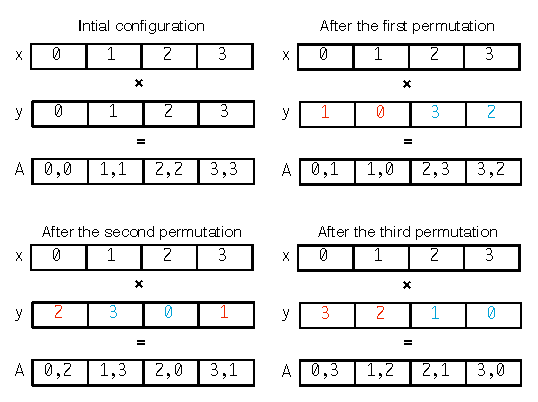
\includegraphics[scale=0.6]{Pictures/vect-by-vect.pdf}}
\caption{Outer-product vectorization by permuting values in a vector register.}
\label{fig:vect-by-vect}
\end{figure}

The storage layout of $A$, however, is incorrect after the application of this ``outer-product vectorization'' ($op$-$vect$). We efficiently restore it with a sequence of vector shuffles following the pattern highlighted in Figure~\ref{fig:restore-layout}, executed once outside of the $ijk$ loop nest. The generated pseudo-code for the simple Helmholtz problem when using $op$-$vect$ is shown in Figure~\ref{code:helmholtz-opvect}.

\begin{figure}[t]
\centerline{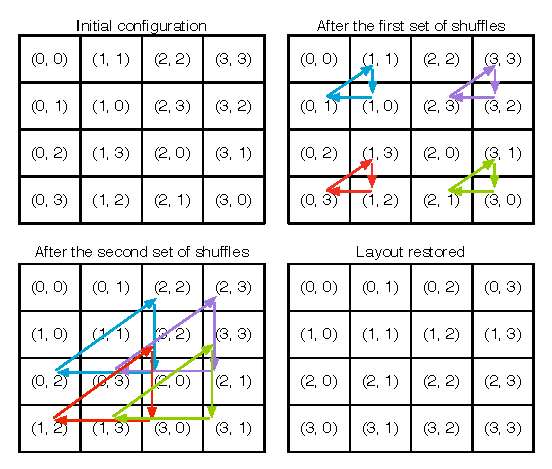
\includegraphics[scale=0.7]{Pictures/vect-restore.pdf}}
\caption{Restoring the storage layout after $op$-$vect$. The figure shows how 4$\times$4 elements in the top-left block of the stiffness matrix $A$ can be brought to their correct positions.}
\label{fig:restore-layout}
\end{figure}

%are sufficiently large to prevent register reuse along the innermost dimension $k$. A combination of the two scenarios is also possible. We want to exploit the small size of the iteration space and the structure of the computation to optimize register management.

\begin{algorithm}[t]
\small
\KwSty{void} helmholtz(double A[8][8], double **coords) $\lbrace$\\
~~// K, det = Compute Jacobian (coords) \\
~~// Declaration of basis function matrices \\
~~\\
~~\KwSty{for} (\KwSty{int} i = 0; i$<$6; i++) $\lbrace$ \\
~~~~// Do loop-invariant code motion \\
~~~~\KwSty{for} (\KwSty{int} j = 0; j$<$4; j+=4) \\
~~~~~~\KwSty{for} (\KwSty{int} k = 0; k$<$8; k+=4) $\lbrace$\\
~~~~~~~~// Call $Load$ and $set$ intrinsics \\
~~~~~~~~// Compute A[1,1],A[2,2],A[3,3],A[4,4] \\
~~~~~~~~// One $permute\_pd$ intrinsics per $k$-loop $load$\\
~~~~~~~~// Compute A[1,2],A[2,1],A[3,4],A[4,3] \\
~~~~~~~~// One $permute2f128\_pd$ intrinsics per $k$-loop $load$\\
~~~~~~~~// ...\\
~~~~~~$\rbrace$\\
~~~~// Do Remainder loop (from $j=4$ to $j=6$)\\
~~$\rbrace$\\
~~// Restore the storage layout:\\
~~\KwSty{for} (\KwSty{int} j = 0; j$<$4; j+=4) $\lbrace$\\
~~~~$\_\_$m256d r0, r1, r2, r3, r4, r5, r6, r7;\\
~~~~\KwSty{for} (\KwSty{int} k = 0; k$<$8; k+=4) $\lbrace$\\
~~~~~~r0 = $\_$mm256$\_$load$\_$pd ($\&$A[j+0][k]);\\
~~~~~~// Load A[j+1][k], A[j+2][k], A[j+3][k]\\
~~~~~~r4 = $\_$mm256$\_$unpackhi$\_$pd (r1, r0);\\
~~~~~~r5 = $\_$mm256$\_$unpacklo$\_$pd (r0, r1);\\
~~~~~~r6 = $\_$mm256$\_$unpackhi$\_$pd (r2, r3);\\
~~~~~~r7 = $\_$mm256$\_$unpacklo$\_$pd (r3, r2);\\
~~~~~~r0 = $\_$mm256$\_$permute2f128$\_$pd (r5, r7, 32);\\
~~~~~~r1 = $\_$mm256$\_$permute2f128$\_$pd (r4, r6, 32);\\
~~~~~~r2 = $\_$mm256$\_$permute2f128$\_$pd (r7, r5, 49);\\
~~~~~~r3 = $\_$mm256$\_$permute2f128$\_$pd (r6, r4, 49);\\
~~~~~~$\_$mm256$\_$store$\_$pd ($\&$A[j+0][k], r0);\\
~~~~~~// Store A[j+1][k], A[j+2][k], A[j+3][k]\\
~~~~$\rbrace$\\
~~$\rbrace$\\
$\rbrace$
\caption{Local assembly code generated by Firedrake when padding, data alignment, $licm$ and $op$-$vect$ are applied to the Helmholtz problem given in Figure~\ref{code:helmholtz}. Here, we assume the polynomial order is $p=2$, since $op$-$vect$ can not be used when an iteration space dimension is smaller than the vector length. The original size of the $j$-$k$ iteration space (i.e. before padding was applied) was 6$\times$6. In this example, the unroll-and-jam factor is 1.}
\label{code:helmholtz-opvect}
\end{algorithm}


% Splitting
\subsection{Expression Splitting}
In complex kernels, like Burgers' in Figure~\ref{code:burgers}, and on certain architectures, achieving effective register allocation can be challenging. If the number of variables independent of the innermost-loop dimension is close to or greater than the number of available CPU registers, it is likely to obtain poor register reuse. This usually happens when the number of basis function matrices, temporaries introduced by loop-invariant code motion, and problem constants is large. For example, applying loop-invariant code motion to Burgers on a 3D mesh needs 33 temporaries for the $ijk$ loop order, and compiler's hoisting of invariant loads out of the $k$ loop can be inefficient on architectures with a relatively low number of registers. One potential solution to this problem consists of suitably ``splitting'' the computation of the stiffness matrix $A$ into multiple sub-expressions; an example, for the simpler Helmholtz problem, is given in Figure~\ref{code:helmholtz-split}. Splitting an expression has, in general, several drawbacks. Firstly, it increases the number of accesses to $A$ proportially to the ``split factor'', which is the number of sub-expressions produced. Secondly, depending on how the split is executed, it can lead to redundant computation (e.g. the product $det*W3[i]$ is performed times number of sub-expressions in the code of Figure~\ref{code:helmholtz-split}). Finally, it might affect register locality, although this is not the case of the Helmholtz example: for instance, the same matrix could be accessed in different sub-expressions, requiring a proportional number of loads be performed. Nevertheless, as shown in Section~\ref{sec:perf-results}, the performance gain from improved register reuse along inner dimensions can still be greater, especially if the split factor and the splitting itself use heuristics to minimize the aforementioned issues.


\begin{algorithm}[t]
\small
\KwSty{void} helmholtz(double A[3][4], double **coords) $\lbrace$\\
~~\KwSty{$\#$define} ALIGN $\_\_$attribute$\_\_$((aligned(32))) \\
~~// K, det = Compute Jacobian (coords) \\
~~// Declaration of basis function matrices \\
~~\\
~~\KwSty{for} (\KwSty{int} i = 0; i$<$3; i++) $\lbrace$ \\
~~~~double LI$\_$0[4];\\
~~~~double LI$\_$1[4];\\
~~~~\KwSty{for} (\KwSty{int} r = 0; r$<$4; r++) $\lbrace$ \\
~~~~~~LI$\_$0[r] = ((K1*X$\_$D10[i][r])+(K3*X$\_$D01[i][r]));\\
~~~~~~LI$\_$1[r] = ((K0*X$\_$D10[i][r])+(K2*X$\_$D01[i][r]));\\
~~~~$\rbrace$\\
~~~~\KwSty{for} (\KwSty{int} j = 0; j$<$3; j++) \\
~~~~~~\KwSty{$\#$pragma vector aligned}\\
~~~~~~\KwSty{for} (\KwSty{int} k = 0; k$<$4; k++) \\
~~~~~~~~A[j][k] += (Y[i][k]*Y[i][j]+LI$\_$0[k]*LI$\_$0[j])*det*W3[i];\\
~~~~\KwSty{for} (\KwSty{int} j = 0; j$<$3; j++) \\
~~~~~~\KwSty{$\#$pragma vector aligned}\\
~~~~~~\KwSty{for} (\KwSty{int} k = 0; k$<$4; k++) \\
~~~~~~~~A[j][k] += LI$\_$1[k]*LI$\_$1[j]*det*W3[i];\\
~~$\rbrace$\\
$\rbrace$
\caption{Local assembly code generated by Firedrake when $split$ is applied to the optimized Helmholtz problem given in Figure~\ref{code:helmholtz-licm}. In this example, the split factor is 2.}
\label{code:helmholtz-split}
\end{algorithm}

Table~\ref{table:code-transformations} summarizes the code transformations described so far. Given that many of these transformations depend on some parameters (e.g. tile size), we need a mechanism to prune such a large space of optimization. This aspect is treated in Section~\ref{sec:pyop2-compiler}.

\begin{table}[h]
\begin{center}
\begin{tabulary}{1.0\columnwidth}{|C|C|}
\hline
Name (Abbreviation) & Parameter \\\hline\hline
Generalized loop-invariant code motion ($licm$) &   \\ \hline
Padding &  \\ \hline
Data Alignment & \\ \hline
Loop interchange      & loops  \\ \hline
Loop unrolling  & unroll factor \\ \hline
Register tiling & tile size \\ \hline
Outer-product vectorization ($op$-$vect$) & tile size \\ \hline
Assembly splitting ($split$) & split point, split factor \\ \hline
\end{tabulary}
\end{center}
\caption{Overview of code transformations for Firedrake-generated assembly kernels.}
\label{table:code-transformations}
\end{table}

% mention (obvious) composability

\section{Overview of the XY Compiler}
\label{sec:pyop2-compiler}
%Design and structure of the PyOP2 Compiler. Show the steps through which the IR is transformed (need to cite Firedrake here). Briefly describe a simple cost model that allows us to prune the space of code transformations.

\begin{algorithm}[t]
\label{algo:PyOP2Compiler}
  \textbf{The XY Compiler}\\
  \KwIn{ast, wrapper, isa}
  \KwOut{code}
// Analyze ast and build optimization plan \\
it\_space = analyze(ast) \\
\If{\KwSty{not} it\_space}{
  ast.apply\_inter\_kernel\_vectorization(wrapper, isa)
  \Return{wrapper + ast.from\_ast\_to\_c()}
}
\If{isa.backend == gpu}{
  \If{it\_space}{ast.extract\_iteration\_space(wrapper)}
  \Return{wrapper + ast.from\_ast\_to\_c()}
}
plan = cost\_model(it\_space.n\_inner\_arrays, isa.n\_regs) \\
// Optimize ast based on plan \\
ast.licm() \\
ast.padding() \\
ast.data\_align() \\
\If{plan.permute}{
  ast.permute\_assembly\_loops()
}
\If{plan.sz\_split}{
  ast.split(plan.sz\_split)
}
\If{plan.uaj\_factor}{
  uaj = MIN(plan.uaj\_factor, $\lfloor$it\_space.j.size/isa.vf$\rfloor$) \\
  ast.op\_vect(uaj)
}
\Return{wrapper + ast.from\_ast\_to\_c()}
\caption{Pseudocode of the XY pipeline.}
\end{algorithm}

Firedrake provides users with the Unified Form Language to write problems in a notation resembling mathematical equations. This high-level specification is translated by the Fenics Form Compiler~\cite{FFC-Compiler} into an Abstract Syntax Tree representation of a Finite Element assembly kernel. ASTs are then passed to PyOP2~\cite{pyop2isc}, which lies at the core of Firedrake, where parallel execution over the unstructured mesh is managed. Our compiler, capable of applying the transformations described in Section~\ref{sec:code-transf}, is integrated with PyOP2: it receives FFC's ASTs as input, it introduces optimizations, and it generates C code as output, which is eventually just-in-time compiled on the underlying architecture. Because of the large number of (possibly parametric) transformations, we need a mechanism to select the most suitable optimization strategy for a given problem. Autotuning might be used, although at the moment we avoid it to minimize the run-time overhead. Our optimization strategy, based on heuristics and a simple cost model, is described in the following, along with an overview of our compiler.

The compiler structure is outlined in Figure~\ref{algo:PyOP2Compiler}. Initially, an AST is inspected, looking for the presence of iteration spaces and other domain-specific information provided by the higher layer. If the kernel lacks an iteration space, then so-called inter-kernel vectorization, in which the non-affine loop over mesh elements is vectorized, can be applied. This feature, currently under development, has been proved to be useful in several Finite-Volume-based applications~\cite{inter-kernel-vect}. The second transformation step is applied if the backend is a manycore machine, like a GPU: the compiler tries to extract parallelism from inside the kernel, by partitioning loop iterations among different threads, if these are found to be independent~\cite{quadrature-cuda}. Then, an ordered sequence of optimization steps are executed. Application of $licm$ must precede padding and data alignment, due to the introduction of temporary arrays. Based on a cost model, the $split$ and $op$-$vect$ transformations may be introduced; their implementation is based on analysis and trasformation of the AST. When $op$-$vect$ is selected, the compiler outputs proper AVX (or LRbi) intrinsics code. Any possible corner cases are handled: for example, if $op$-$vect$ is to be applied, but the size of the iteration space is not a multiple of the vector length, then a reminder loop, amenable to auto-vectorization, is inserted. 

The cost model is shown in Figure~\ref{algo:applyCostModel}. It takes into account the number of available logical vector registers ($n\_regs$) and the number of variables iterating along the $j$ and $k$ dimensions ($n\_consts$ for independent variables, $n\_outer\_arrays$ for $j$ variables, and $n\_inner\_arrays$ for $k$ variables, assuming the $ijk$ loop order) to estimate unroll-and-jam and split factors when, respectively, $op$-$vect$ and $split$ are used. The $n\_consts$ parameter includes temporary registers to carry out computations, so setting its value is partly driven by heuristics. If a factor is 0, then the corresponding transformation is not applied. The $split$ transformation is triggered whenever the number of hoistable terms is larger than the available registers along the outer dimension (lines 3-8), which is approximated as half of the total (line 2). A split factor of $n$ means that the assembly expression should be ``cut'' into $n$ sub-expressions. Depending on the structure of the assembly expression, each sub-expression might end up accessing a different number of arrays; the cost model is simplified by assuming that all sub-expressions are of the same size. Finally, the unroll-and-jam factor for the $op$-$vect$ transformation is determined as a function of the available registers, i.e. those not used for storing hoisted terms (line 9-11). 

Loop unroll and unroll-and-jam of outer loops are fundamental to expose ILP and data reuse, and so tuning critical parameters, like the unroll factor, becomes of great importance. It is our experience (inspection of assembly code, comparison with other hand-made implementations), however, that for assembly kernels, where the loop nest is affine, bounds are known at compile-time, and memory accesses are unit-stride, recent versions of a vendor compiler like $intel$'s (or $icc$) employ cost models capable of estimating close-to-optimal values for such parameters. We leave therefore the backend compiler in charge to select unroll and unroll-and-jam factors. This choice also simplifies the compiler's cost model. The only situation in which we explicitly unroll-and-jam a loop is when $op$-$vect$ is used, since the transformed code seems to prevent the $icc$ compiler from applying unroll-based optimizations, even if specific pragmas are added. Note that, regardless of the output of the cost model, the unroll-and-jam factor never exceeds the actual size of the outer loop (line 25 in Figure~\ref{algo:PyOP2Compiler}, assuming the default loop order $ijk$).

All loops are interchangeable provided that temporaries are introduced if the nest is not perfect. For the employed storage layout, the loop permutations $ijk$ and $ikj$ are likely to maximize performance. Conceptually, this is motivated by the fact that if the $i$ loop were in an inner position, then a significantly higher number of load instructions would be required every iteration; experiments showed that the performance loss is greater than the gain due to the possibility of accumulating increments in a register, rather than in memory, along the $i$ loop. The choice between $ijk$ and $ikj$ depends on the number of load instructions that can be hoisted out of the innermost dimension. Our compiler chooses, as outer, the loop along which the number of invariant loads is smaller so that more registers are availabe to carry out the computation of the stiffness matrix. 


\begin{algorithm}[t]
\label{algo:applyCostModel}
  \textbf{Cost Model}\\
  \KwIn{n\_outer\_arrays, n\_inner\_arrays, n\_consts, n\_regs}
  \KwOut{uaj\_factor, split\_factor}

n\_outer\_regs = n\_regs / 2 \\
split\_factor = 0 \\ 
// Compute spltting factor \\
\While{n\_outer\_arrays $>$ n\_outer\_regs}{
  n\_outer\_arrays = n\_outer\_arrays / 2 \\
  split\_factor = split\_factor + 1 
}

// Compute unroll-and-jam factor for $op$-$vect$ \\
n\_regs\_avail = n\_regs - (n\_outer\_arrays + n\_consts)\\
uaj\_factor = $\lceil$n\_reg\_avail / n\_inner\_arrays$\rceil$ \\
\Return{$<$split\_factor, uaj\_factor$>$}
\caption{The cost model is employed by the compiler to estimate the most suitable unroll-and-jam (when $op$-$vect$ is used) and split factors, avoiding the overhead of auto-tuning.}
\end{algorithm}


\section{Performance Evaluation}
\label{sec:perf-results}

\subsection{Experimental Setup}
Experiments were run on two Intel machines, a Sandy Bridge (I7-2600 CPU, running at 3.4GHz, 32KB L1 cache and 256KB L2 cache) and the Phi. The \texttt{icc 2013} compiler was used, with optimization level \texttt{-O2} and with auto-vectorization enabled (\texttt{-xAVX} on the Sandy Bridge, and \texttt{TODO} on the Phi). Other optimization levels performed, in general, slightly worse than \texttt{-O2}. Our code transformations were evaluated in three real-world problems based on the following PDEs:
\begin{itemize}
\item Helmholtz
\item Advection-Diffusion
\item Burgers
\end{itemize}
The code was written in UFL and then executed over real unstructured meshes through Firedrake. The Helmholtz code has already been shown in Figure~\ref{code:helmholtz}. For Advection-Diffusion, the ``Diffusion'' equation, which uses the same differential operators as Helmholtz, is considered. In the Diffusion kernel, the main differences with respect to Helmholtz are the absence of the $Y$ array and the presence of a few more constants for computing the stiffness matrix $A$. Burgers is a time-dependent problem, i.e. the assembly is recalculated every time step based on the result of previous iterations. It employs differential operators different from those of Helmholtz, which has a major impact on the generated assembly code (Figure~\ref{code:burgers}), where a larger number of basis function matrices ($X1$, $X2$, ...) and constants ($F0$, $F1$, ..., $K0$, $K1$, ...) are accessed. 

These problems were studied varying both the shape of mesh elements and the polynomial order $p$ of the method. Intuitively, the larger the element shape, the bigger is the iteration space. Triangles (2D), tetrahedron (3D), and prisms (3D) were tested. For instance, in the case of Helmholtz with $p=1$, the size of the $j$ and $k$ loops for the three kind of elements is, respectively, $3$, $4$, and $6$. Moving from 2D to 3D also increases the number of basis function arrays, since conceptually the behaviour of the equation has to be approximated also along the $z$ dimension. On the other hand, the polynomial order affects only the problem size (the three loops $i$, $j$, and $k$, and, as a consequence, the size of $X$ and $Y$ arrays). A range of polynomial orders, from $p=1$ to $p=4$, are tested; higher polynomial orders are excluded from the study because of current Firedrake limitations. In such a large space of problems, the size of the stiffness matrix rarely excees 20$\times$20, with a peak of 105$\times$105 in Burgers with prisms and $p=4$. 

For the Helmholtz 3D problem, manual implementations based on MKL BLAS were tested on Sandy Bridge. This particular kernel can be easily reduced to a sequence of four matrix-matrix multiplications that can be computed via calls to BLAS \texttt{dgemm}. In the case of $p=4$, where the stiffness matrix is of size 35$\times$35, the computation was almost twice slower than the case in which only $licm$, data alignment and padding were used. As anticipated, extraction of matrix-matrix multiplications from analysis of the kernel's AST or re-design of the Fenics Form Compiler to explicitly expose these operations will be addressed in further work. However, these experiments justify that there is a set of problems for which turning to BLAS is not beneficial in terms of performance. It is possible that employing BLAS is useful for particularly large problems, for instance Burgers on 3D meshes with $p \geq 3$, although the loss in data locality due to re-loading matrices appearing in multiple products might limit the performance gain. 

\subsection{Impact of Generalized Loop-invariant Code Motion}
\newcommand{\massmatrixtwodresultsnorms}{
\begin{tabularx}{1.0\textwidth}{p{3.5cm}p{3.5cm}|p{2.25cm}p{2.25cm}p{2.25cm}p{2.25cm}|}
\cline{3-6}
& & \multicolumn{2}{c|}{\texttt{AVX}} & \multicolumn{2}{c|}{\texttt{Phi}}\\
\cline{3-6}
& & \multicolumn{1}{c}{\texttt{licm}} & \multicolumn{1}{c|}{\texttt{licm+ap}} & \multicolumn{1}{c}{\texttt{licm}} & \multicolumn{1}{c|}{\texttt{licm+ap}} \\
\cline{1-6}
\multicolumn{1}{|c|}{\texttt{Helmholtz}} & \multicolumn{1}{c|}{\texttt{triangle}} & ~~1.34$\times$-4.32$\times$ & ~1.34$\times$-4.32$\times$ & ~~1.34$\times$-4.32$\times$ & ~1.34$\times$-4.32$\times$ \\
\multicolumn{1}{|c|}{\texttt{Helmholtz}} & \multicolumn{1}{c|}{\texttt{tetrahedron}} & 1.34$\times$-4.32$\times$ & 1.34$\times$-4.32$\times$ & 1.34$\times$-4.32$\times$ & 1.34$\times$-4.32$\times$ \\
\multicolumn{1}{|c|}{\texttt{Helmholtz}} & \multicolumn{1}{c|}{\texttt{prism}} & 1.34$\times$-4.32$\times$ & 1.34$\times$-4.32$\times$ & 1.34$\times$-4.32$\times$ & 1.34$\times$-4.32$\times$ \\
\cline{1-6}
\multicolumn{1}{|c|}{\texttt{Diffusion}} & \multicolumn{1}{c|}{\texttt{triangle}} & 1.34$\times$-4.32$\times$ & 1.34$\times$-4.32$\times$ & 1.34$\times$-4.32$\times$ & 1.34$\times$-4.32$\times$ \\
\multicolumn{1}{|c|}{\texttt{Diffusion}} & \multicolumn{1}{c|}{\texttt{tetrahedron}} & 1.34$\times$-4.32$\times$ & 1.34$\times$-4.32$\times$ & 1.34$\times$-4.32$\times$ & 1.34$\times$-4.32$\times$ \\
\multicolumn{1}{|c|}{\texttt{Diffusion}} & \multicolumn{1}{c|}{\texttt{prism}} & 1.34$\times$-4.32$\times$ & 1.34$\times$-4.32$\times$ & 1.34$\times$-4.32$\times$ & 1.34$\times$-4.32$\times$ \\
\cline{1-6}
\multicolumn{1}{|c|}{\texttt{Burgers}} & \multicolumn{1}{c|}{\texttt{triangle}} & 1.34$\times$-4.32$\times$ & 1.34$\times$-4.32$\times$ & 1.34$\times$-4.32$\times$ & 1.34$\times$-4.32$\times$ \\
\multicolumn{1}{|c|}{\texttt{Burgers}} & \multicolumn{1}{c|}{\texttt{tetrahedron}} & 1.34$\times$-4.32$\times$ & 1.34$\times$-4.32$\times$ & 1.34$\times$-4.32$\times$ & 1.34$\times$-4.32$\times$ \\
\multicolumn{1}{|c|}{\texttt{Burgers}} & \multicolumn{1}{c|}{\texttt{prism}} & 1.34$\times$-4.32$\times$ & 1.34$\times$-4.32$\times$ & 1.34$\times$-4.32$\times$ & 1.34$\times$-4.32$\times$ \\
\cline{1-6}
\end{tabularx}
}

\begin{table*}[t]\normalsize
\massmatrixtwodresultsnorms
\label{table:perf-results-licm-helmholtz}
\caption{Impact of generalized loop-invariant code motion ($licm$ column) on the Helmholtz, Diffusion and Burgers problems, for three kind of elements belonging to the Lagrange family (triangle, tetrahedron, prism), for the range of polynomial orders $p$ $\in$ $\lbrace$1, 4$\rbrace$. Each entry indicates the range of speed-ups obtained over the non-optimized implementation. The column $licm$-$ap$ illustrates the combination of $licm$ with data alignment and padding. Results are shown for both the Sandy Bridge and the Phi machine.}
\end{table*}

Tables~\ref{table:perf-results-licm-helmholtz},~\ref{table:perf-results-licm-advdiff}, and~\ref{table:perf-results-licm-burgers} illustrate the speed-ups obtained on the Sandy Bridge and the Phi machines when $licm$, data alignment, and padding are used, over non-transformed code. Inspection of assembly code generated by $icc$ confirmed all limitations described in Section~\ref{sec:code-transf-licm}: only sub-expressions invariant with respect to outer loops are hoisted and, interestingly, not vectorized. This motivates the usually significant gain. Padding and data alignment enhance, in general, the quality of SIMD auto-vectorization. As shown in Figure~\ref{algo:PyOP2Compiler}, these transformations are applied on top of $licm$, so we refer to them as $licm$-$ap$. Sometimes the run-time of $licm$-$ap$ is similar to that of $licm$ because the stiffness matrix size is, without padding, already a multiple of the vector length, and data is automatically aligned. Occasionally $licm$-$ap$ is slower than $licm$ (e.g. in Burgers 3D p3). This is due to the large number of aligned temporaries introduced by $licm$, which probably leads to cache associativity conflicts. 

\subsection{Impact of Vector-register Tiling}
Figures~\ref{fig:opvect-helmholtz-speedup},~\ref{fig:opvect-diffusion-speedup}, and~\ref{fig:opvect-burgers-speedup} show the speed-ups achieved by applying $op$-$vect$ on top of $licm$-$ap$ to the Helmoltz, Diffusion, and Burgers assembly kernels, respectively. For each problem instance we report the best run-time obtained by empirically testing a set of different unroll/unroll-and-jam factors, and the one retrieved through the XY's cost model.

% why better results at higher order

\subsection{Impact of Expression Splitting}
% why split useless in helmholtz/diffusion
% why vect vect+split useless in burgers




\begin{figure}[h]
\centerline{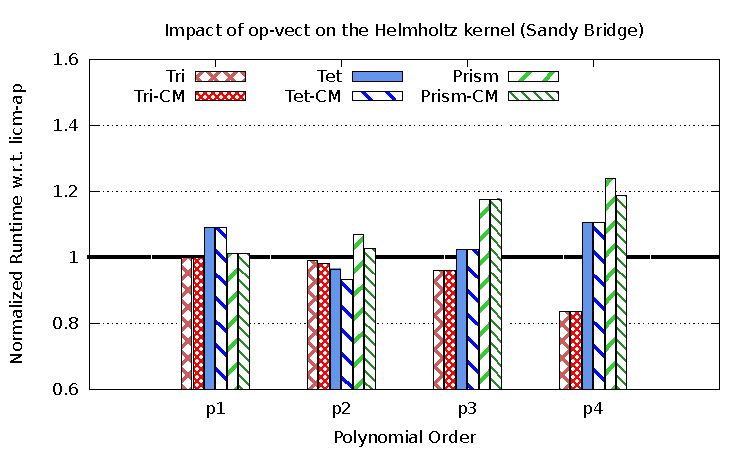
\includegraphics[scale=0.7]{Pictures/helmholtz-normalized-opvect.pdf}
\label{fig:opvect-helmholtz-speedup}}
\caption{Speed-ups obtained by applying $op$-$vect$ on top of $licm$-$ap$ to the Helmholtz kernel.}
\end{figure}

\begin{figure}[h]
\centerline{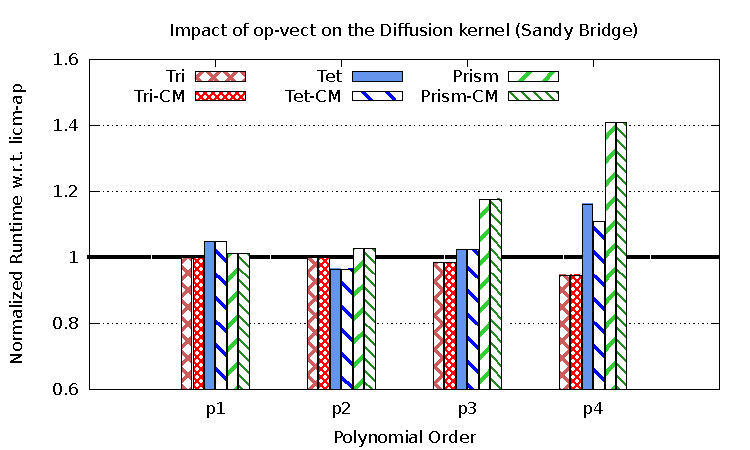
\includegraphics[scale=0.7]{Pictures/diffusion-normalized-opvect.pdf}
\label{fig:opvect-diffusion-speedup}}
\caption{Speed-ups obtained by applying $op$-$vect$ on top of $licm$-$ap$ to the Diffusion kernel.}
\end{figure}

\begin{figure}[h]
\centerline{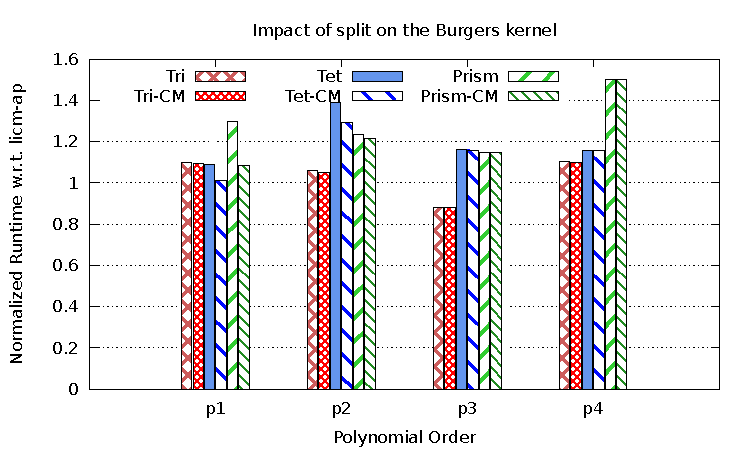
\includegraphics[scale=0.7]{Pictures/burgers-normalized-split.pdf}
\label{fig:opvect-burgers-speedup}}
\caption{Speed-ups obtained by applying $op$-$vect$ on top of $licm$-$ap$ to the Burgers kernel.}
\end{figure}


\section{Related Work}
\label{sec:related-work}
The finite element method is used in the most disparate contexts to approximate solutions of PDEs. Well-known frameworks and applications include nek5000~\cite{nek5000-web-page}, the Fenics project~\cite{Fenics}, Fluidity~\cite{fluidity_manual_v4}, and of course Firedrake; this is not an exhaustive list, though. Numerical integration is usually employed to implement the local assembly phase. The recent introduction of DSLs to decouple the finite element specification from its underlying implementation facilitated, however, the development of novel approaches. Methods based on tensor contraction~\cite{FFC-TC} and symbolic manipulation~\cite{Francis} have been developed, although it has been demonstrated that numerical integration remains the optimal choice for a wide class of problems~\cite{quadrature1}. 

Optimization of local assembly using numerical integration for CPU platforms has been tackled in~\cite{quadrature1}. However, to the best of our knowledge, ours is the first work targeting low-level optimizations and adopting a real compiler approach. In~\cite{Markall20101815}, and more recently in~\cite{petsc-integration-gpu}, the problem has been studied for GPU architectures. In~\cite{assembly-opencl}, variants of the standard numerical integration algorithm have been specialized for the PowerXCell processor and evaluated; The paper lacks, however, an exhaustive study from the compiler viewpoint as we did, and none of the optimizations presented in Section~\ref{sec:code-transf} are mentioned. 

Domain-specific languages and automated code generation have been adopted with success in different areas. Spiral~\cite{Pueschel:05} automates generation of highly-optimized platform-specific digital signal processing numerical algorithms. Similar ideas are adopted in~\cite{Spampinato:14}, where a DSL and a compiler for dense linear algebra kernels are proposed. OP2~\cite{op2-main}, and its python implementation~\cite{pyop2isc}, which is used by Firedrake to express iteration over meshes, aim at achieving performance portability for scientific codes based on unstructured meshes. Stencil DSLs and compilers, such as Pochoir~\cite{pochoir} and SDSL~\cite{stencil-compiler}, have been developed to support development and high performance in fields like image processing and scientific computations over structured grids.  

XY currently uses a simple cost model and heuristics to steer the optimization process. Many code generators, like those based on the Polyhedral model~\cite{PLUTO} and those driven by domain-knowledge~\cite{modeldriven}, make use of cost models. The other extreme consists of relying on auto-tuning to select the best implementation for a given problem on a certain platform. Notable examples include tuning of small matrix-matrix multiplies in nek5000~\cite{nek5000}, the ATLAS library~\cite{ATLAS}, and FFTW~\cite{FFTW} for fast fourier transforms. In both cases, pruning the implementation space, as we did in Section~\ref{sec:pyop2-compiler}, is fundamental to mitigate complexity and overhead. 

%(i.e. given a mesh, those that lead to ``less accurate'' solutions than when using high-order polynomials, at a lower computational cost)

%Show other work of people working on optimizations for computational science kernels. Inter-kernel vectorisation paper from Istvan. Previous work in FFC. Spencer et-al + Shin et. al. attempt to optimize computations that could benefit from using BLAS, but in practice they don't, due to the very small dgemm operations employed. Saday's model-driven SIMD code vectorisation for the tensor contraction engine.


\section{Conclusions}
\label{sec:conclusions}

In this paper we have presented design, optimizations and systematic performance evaluation of XY, a compiler for finite element local assembly. In this context, to the best of our knowledge, this is the first compiler oriented towards the introduction of low-level optimizations to maximize instruction-level parallelism, register locality and SIMD vectorization. Assembly kernels have peculiar characteristics. Their iteration space is usually very small, with the size depending on aspects like the degree of accuracy one wants to reach (polynomial order of the method) and the mesh discretization employed. The data space, in terms of number of matrices and scalar, grows proportionally to the complexity of the finite element problem. XY has been developed taking into account all of these aspects, knowing that some transformations are useful only in a subset of all possible problems. The various optimizations overcome limitations of current vendor and research compilers. The exploitation of domain-knowledge allows some of them to be particularly effective, as demonstrated by our experiments on two state-of-the-art Intel platforms. Further work include a comprehensive study about feasibility and constraints of transforming the kernel into a sequence of BLAS calls. XY supports all of the problems expressible in Firedrake, and it is already integrated with this framework. 



% use section* for acknowledgement
\section*{Acknowledgment}

This research is partly funded by the MAPDES project and by the Department of Computing at Imperial College London. The authors would like to thank Prof. J. Ramanujam for his invaluable suggestions, and Dr. Lawrence Mitchell and Dr. Francis Russell for their contribution to the PyOP2 project.


%\newcommand{\massmatrixtwodresultsnorms}{
%\begin{tabularx}{1.0\textwidth}{p{3.5cm}|p{1.98cm}p{1.98cm}p{1.98cm}|p{1.98cm}p{1.98cm}p{1.98cm}|}
%\cline{2-7}
%& \multicolumn{3}{c|}{\texttt{AVX}} & \multicolumn{3}{c|}{\texttt{PHI}} \\
%\cline{2-7}
%& \texttt{original} & \texttt{licm} & \texttt{licm+ap} & \texttt{original} & \texttt{licm} & \texttt{licm+ap}\\
%\cline{1-7}
%\multicolumn{1}{|c|}{\texttt{triangle p1}} & $5.49e{-}17$ & $4.95e{-}17$ & $1.44e{-}17$ & $1.34e{-}17$ & $1.56e{-}17$ & $\mathbf{4.43e{-}5}$ \\
%\multicolumn{1}{|c|}{\texttt{triangle p2}} & $5.49e{-}17$ & $4.95e{-}17$ & $1.44e{-}17$ & $1.34e{-}17$ & $1.56e{-}17$ & $\mathbf{4.43e{-}5}$ \\
%\multicolumn{1}{|c|}{\texttt{triangle p3}} & $5.49e{-}17$ & $4.95e{-}17$ & $1.44e{-}17$ & $1.34e{-}17$ & $1.56e{-}17$ & $\mathbf{4.43e{-}5}$ \\
%\multicolumn{1}{|c|}{\texttt{triangle p4}} & $5.49e{-}17$ & $4.95e{-}17$ & $1.44e{-}17$ & $1.34e{-}17$ & $1.56e{-}17$ & $\mathbf{4.43e{-}5}$ \\
%\cline{1-7}
%\multicolumn{1}{|c|}{\texttt{tetrahedron p1}} & $5.49e{-}17$ & $4.95e{-}17$ & $1.44e{-}17$ & $1.34e{-}17$ & $1.56e{-}17$ & $\mathbf{4.43e{-}5}$ \\
%\multicolumn{1}{|c|}{\texttt{tetrahedron p2}} & $5.49e{-}17$ & $4.95e{-}17$ & $1.44e{-}17$ & $1.34e{-}17$ & $1.56e{-}17$ & $\mathbf{4.43e{-}5}$ \\
%\multicolumn{1}{|c|}{\texttt{tetrahedron p3}} & $5.49e{-}17$ & $4.95e{-}17$ & $1.44e{-}17$ & $1.34e{-}17$ & $1.56e{-}17$ & $\mathbf{4.43e{-}5}$ \\
%\multicolumn{1}{|c|}{\texttt{tetrahedron p4}} & $5.49e{-}17$ & $4.95e{-}17$ & $1.44e{-}17$ & $1.34e{-}17$ & $1.56e{-}17$ & $\mathbf{4.43e{-}5}$ \\
%\cline{1-7}
%\multicolumn{1}{|c|}{\texttt{prism p1}} & $5.49e{-}17$ & $4.95e{-}17$ & $1.44e{-}17$ & $1.34e{-}17$ & $1.56e{-}17$ & $\mathbf{4.43e{-}5}$ \\
%\multicolumn{1}{|c|}{\texttt{prism p2}} & $5.49e{-}17$ & $4.95e{-}17$ & $1.44e{-}17$ & $1.34e{-}17$ & $1.56e{-}17$ & $\mathbf{4.43e{-}5}$ \\
%\multicolumn{1}{|c|}{\texttt{prism p3}} & $5.49e{-}17$ & $4.95e{-}17$ & $1.44e{-}17$ & $1.34e{-}17$ & $1.56e{-}17$ & $\mathbf{4.43e{-}5}$ \\
%\multicolumn{1}{|c|}{\texttt{prism p4}} & $5.49e{-}17$ & $4.95e{-}17$ & $1.44e{-}17$ & $1.34e{-}17$ & $1.56e{-}17$ & $\mathbf{4.43e{-}5}$ \\
%\cline{1-7}
%
%\end{tabularx}
%}
%
%\begin{table*}[t]\normalsize
%\massmatrixtwodresultsnorms
%\label{table:perf-results-licm-helmholtz}
%\caption{Impact of generalized loop-invariant code motion ($licm$ column) on the Helmholtz problem, for three kind of elements belonging to the Lagrange family (triangle, tetrahedron, prism) and for the range of polynomial orders $p$ $\in$ $\lbrace$1, 4$\rbrace$. The column $licm$-$ap$ illustrates the combination of $licm$ with data alignment and padding.}
%\end{table*}


% trigger a \newpage just before the given reference
% number - used to balance the columns on the last page
% adjust value as needed - may need to be readjusted if
% the document is modified later
%\IEEEtriggeratref{8}
% The "triggered" command can be changed if desired:
%\IEEEtriggercmd{\enlargethispage{-5in}}

% references section

% can use a bibliography generated by BibTeX as a .bbl file
% BibTeX documentation can be easily obtained at:
% http://www.ctan.org/tex-archive/biblio/bibtex/contrib/doc/
% The IEEEtran BibTeX style support page is at:
% http://www.michaelshell.org/tex/ieeetran/bibtex/
%\bibliographystyle{IEEEtran}
% argument is your BibTeX string definitions and bibliography database(s)
%\bibliography{IEEEabrv,../bib/paper}
%
%% <OR> manually copy in the resultant .bbl file
%% set second argument of \begin to the number of references
%% (used to reserve space for the reference number labels box)
%\begin{thebibliography}{1}
%
%\bibitem{IEEEhowto:kopka}
%H.~Kopka and P.~W. Daly, \emph{A Guide to \LaTeX}, 3rd~ed.\hskip 1em plus
%  0.5em minus 0.4em\relax Harlow, England: Addison-Wesley, 1999.
%
%\end{thebibliography}
%

\bibliographystyle{plain}	% (uses file "plain.bst")
\bibliography{biblio}		% expects file "myrefs.bib"



% that's all folks
\end{document}


